% after-compact-8.tex

\documentclass[tikz]{standalone}
\usetikzlibrary{decorations.pathreplacing, positioning, arrows.meta, shapes.multipart}

\begin{document}
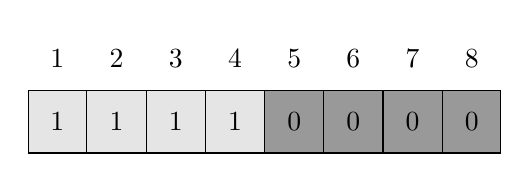
\begin{tikzpicture}[Array/.style = {rectangle split, rectangle split parts = #1, rectangle split horizontal,
    inner sep = 8pt, anchor = center}]
  % list 
  \node[Array = {8}, draw, rectangle split part fill = {gray!20, gray!20, gray!20, gray!20, gray!80}] (L) 
    {1\nodepart{two}1\nodepart{three}1\nodepart{four}1\nodepart{five}0\nodepart{six}0\nodepart{seven}0\nodepart{eight}0};
  % list index
  \node[Array = {8}, above = 0.cm of L] (L-index) 
    {1\nodepart{two}2\nodepart{three}3\nodepart{four}4\nodepart{five}5\nodepart{six}6\nodepart{seven}7\nodepart{eight}8};
\end{tikzpicture}
\end{document}